\chapter{Performance analysis}

\label{Chapter4} 

\section{Creating the benchmark}

\subsection{Lighthouse}

In order to measure the performance of a web site, several techniques exist. One of those is a Lighthouse report. 
This report encompasses lots of different metrics which each tell you more about a website. 
Not all of these metrics are performance metrics, some are an indicator for accessibility, others for search engine optimization or other miscellaneous metrics.
Which metrics we will analyse was expanded upon in the previous chapter but I wanted to reiterate why I chose Lighthouse.

Lighthouse is an open source solution which can be ran locally. 
A lot of alternatives to Lighthouse are proprietary, hosted solutions. 
This makes it a lot harder to benchmark the PoCs because they should all get deployed and be accessible from the internet. 
During development of this benchmark, it helped a lot to be able to instantly run a new benchmark with the new code without having to go through a full deployment.

A negative about Lighthouse is that is difficult to run on browsers other than Google Chrome. While it is technically possible to do so, I did not implement this and opted to use a single browser for testing.

\subsection{Docker}

Docker was used to run the benchmark. Every PoC application has a Dockerfile which details the steps of the build. 
Why use Docker when you could also just run the applications directly on the host?
Because using Docker to create images of the applications makes for a reproducible build and allows me to control every parameter of the process.
In theory, it does not matter whether the images are built on Linux or Windows. 
It does not matter which version of node is locally installed, because the version is specified in the Dockerfile.

Furthermore, Docker not only provides more control over the build, it also gives more control and configurability to the runtime. 
By using Docker Compose, I can dictate how containers can talk to each other.

All of this together makes for a more stable and deterministic build process. 
It allows other people, on different machines, to run the same benchmark easily and observe similar results.

It should be noted that the Dockerfiles for each PoC has some slight differences.
While the PoCs are all websites, running them in Docker is not the same. 
In effect, for the Next PoC, the built-in next web server was used while for the Gatsby PoC, an intermediate container running Nginx was used.

\subsection{Jupyter notebook}

The results of this benchmark are lots of numbers. 
Especially when the benchmark is run several times, it quickly becomes infeasible to manually calculate and create graphs.
I solved this by creating a Jupyter notebook which handles all the calculations and graphing. 
The notebook requires a modern version of Python installed. 
Python 3.8.5 was used for the graphs in this paper but as long as you use at least Python 3, it should work fine.

To run the notebook, a few dependencies are required. 
These can be viewed at the top of the notebook and can be installed with the Python package manager, pip. 


\section{Running the benchmark}

In order to see which of the web technologies scores best, a performance benchmark was created. 
This benchmark uses Cypress to run a Lighthouse report for each PoC application.

The steps for running it are as follows:

\begin{enumerate}
	\item Start the CMS containers.
	      \begin{verbatim}
			docker-compose -f docker-compose-deps.yml up -d
	      \end{verbatim}
	      This will start a Postgres database and Strapi, the CMS. 
	      These must be ran before the others since the build scripts for the web applications require Strapi.
	      The git repo for this paper includes bootstrapped data for Strapi, with a campaign already configured, complete with starting data.
	\item Build all the PoC applications
	      	      	      	      	      	      	      	      	      	      	      	      	      	      	      	      	      	      	      	      	      	      	      	      	      	      	      	      	      	      	      	      	      	      	      	      	      	      	      	
	      \begin{verbatim}
			docker-compose -f docker-compose-bench.yml up -d
	      \end{verbatim}
	      This will build the applications and start the containers. 
	      You can access each application in the browser, starting with port 3000. (http://localhost:3000, http://localhost:3001, \dots)
	      	      	      	      	      	      	      	      	      	      	      	      	      	      	      	      	      	      	      	      	      	      	      	      	      	      	      	      	      	      	      	      	      	      	      	      	      	      	      
	\item  
	      	      	      	      	      	      	      	      	      	      	      	      	      	      	      	      	      	      	      	      	      	      	      	      	      	      	      	      	      	      	      	      	      	      	      	      	      
	      \begin{verbatim}
			cd packages/benchmark
			npm ci
			npm run cypress:open
	      \end{verbatim}
	      	      	      	      	      	      	      	      	      	      	      	      	      	      	      	      	      	      	      	      	      	      	      	      	      	      	      	      	      	      	      	      	      	      	      	      	      
	      This will install Cypress and its dependencies. 
	      After running the final command, Cypress will open and you are able to run the benchmark.
	      Reports with raw data will be saved in the packages/benchmark/reports directory.
\end{enumerate}

These are the steps to run the benchmark once. In order to get a statistically relevant measurement, a script in available that will run the benchmark multiple times.
At the top of the script, you'll find a variable TOTAL\_RUNS which you can adjust and will control how many times the benchmark is ran.
It can be run with

\begin{verbatim}
		cd packages/benchmark
		node runBenchmark.js
\end{verbatim}

Results from these benchmarking runs can be found in the file packages/benchmark/finalReport.json

Finally, you will find a Jupyter notebook that does some number crunching and renders the plots at packages/data-analysis/analysis.ipynb

Results with raw data can be found in appendix \ref{appendix:lighthouse-report}

\section{Largest contentful paint}

\begin{figure}[htb!]
	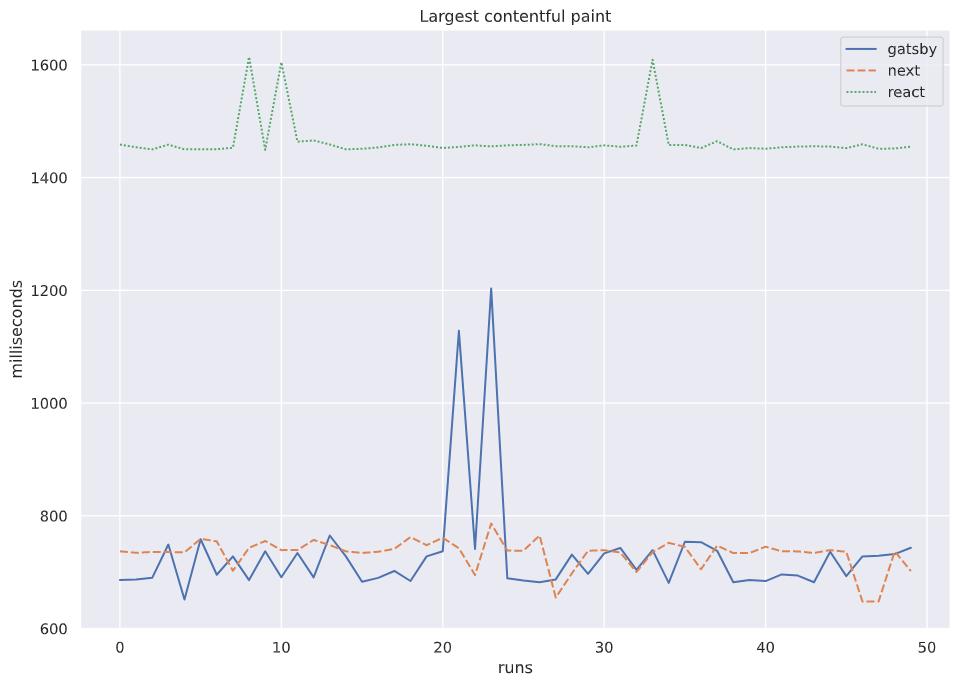
\includegraphics[scale=0.4]{largest_contentful_paint}{}
	\caption{Results of performance benchmark for largest contentful paint}
	\label{fig:largest_contentful_paint}
\end{figure}

In figure \ref{fig:largest_contentful_paint}, it is clear that LCP for a traditional React application is far greater than that of static site generators.

This makes sense: a traditional React application will perform many computational steps during runtime to render the DOM.
Static site generators will perform these computations during the build step.

\section{Total blocking time}


\begin{figure}[htb!]
	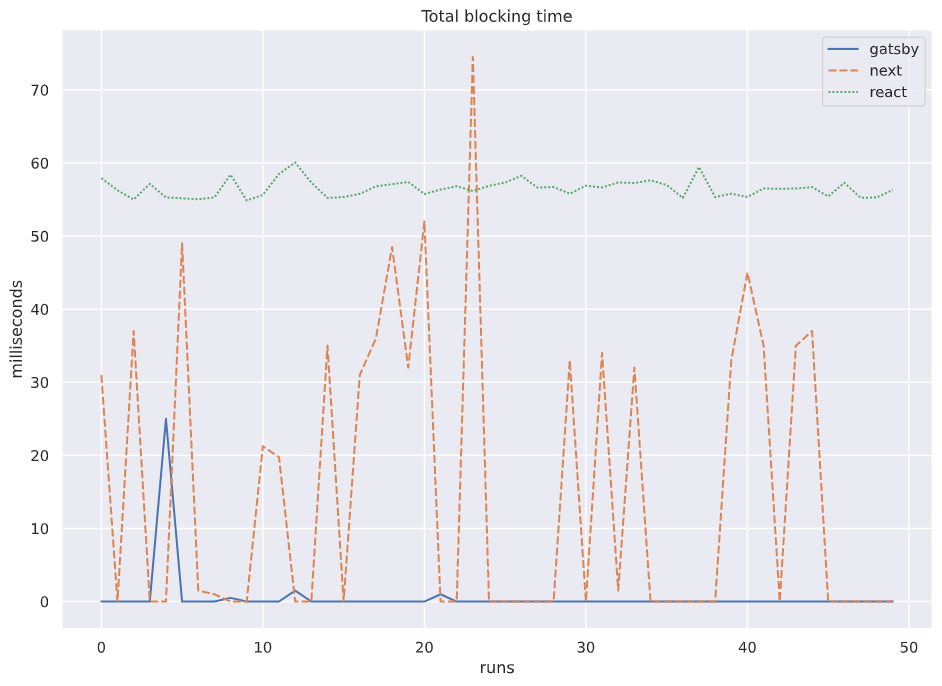
\includegraphics[scale=0.4]{total_blocking_time}
	\caption{Results of performance benchmark for total blocking time}
	\label{fig:total_blocking_time}
\end{figure}

In figure \ref{fig:total_blocking_time}, similar results to the previous figure can be observed
The traditional React application scores much less favorably than the static site generators.
Interestingly, the results for Next seem to spike a lot.


\section{Max potential first input delay}

\begin{figure}[htb!]
	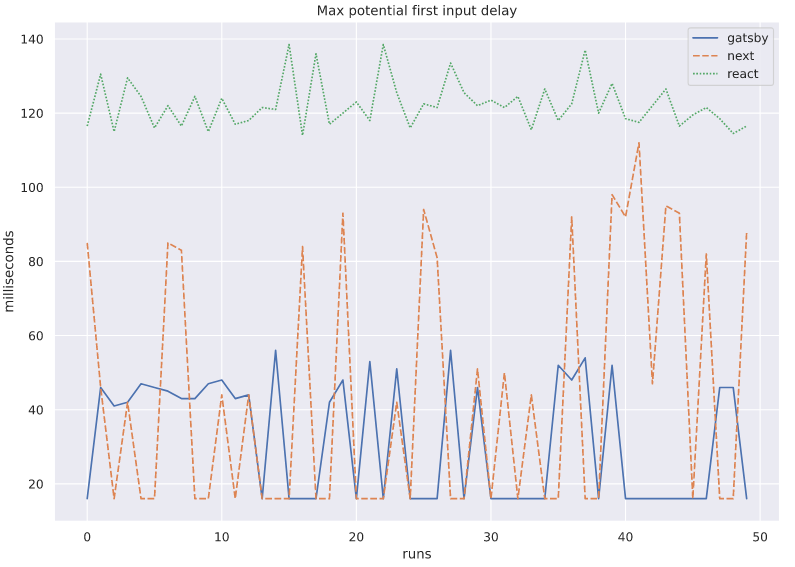
\includegraphics[scale=0.5]{max_potential_first_input_delay}
	\caption{Results of performance benchmark for max potential first input delay}
	\label{fig:max_potential_first_input_delay}
\end{figure}

In figure \ref{fig:max_potential_first_input_delay}, similar results can be observed. 
The traditional React application scores the worst while the static site generators score significantly better.
It's worth noting that all of the PoCs exhibit irregular measurements, FID fluctuates a lot.
However, on average, the Gatsby PoC scores the best for this metric out of all the PoCs.

\section{Bundle size}

To measure the size of the resulting files after a production build was measured with the Unix command 

\begin{verbatim}
	du -c <directory>
\end{verbatim}

\begin{table}[htb!]
	\begin{center}
		\begin{tabular}{||c c||} 
			\hline
			Site   & Size \\ [0.5ex] 
			\hline\hline
			Gatsby & 3072 \\ 
			\hline
			Next   & 7012 \\
			\hline
			React  & 568  \\[1ex] 
			\hline
		\end{tabular}
		\caption{Total file size of production builds, in kilobytes }
		\label{tbl:bundle_size}
	\end{center}
\end{table}

Looking at table \ref{tbl:bundle_size}, the traditional React application has the smallest bundle here. 
This makes sense, the static generators Next and Gatsby will bundle assets while the traditional React app will fetch these during runtime.

While these results are interesting to see, it should not be a definite factor when deciding which technology to use.
The PoCs created for this paper are very small, a real application would have orders of magnitude more lines of code.
Minification really shines with larger codebases. 